\section{Feature Definitions}
\label{section:definitions}
Here, an overview of the algorithms used by the \textit{Mobility Features Package} will be provided. The overview will not discuss implementation details but will provide precise definitions for how these are computed and the considerations which were made. Most of the features were simple to implement with support for real-time computation and were just a matter of performing arithmetic with regards to distance and time spent and places, however, the ones which need some explanation are outlined in this section. 

The Mobility Features included in the Mobility Features package are a subset of the features described by Saeb et al. \cite{Saeb2015}, Canzian et al. \cite{Canzian2015} and Cuttone et al. \cite{sparse-location-2014} and are outlined in Table \ref{tab:features-nilsson}.

\begin{table}[h]
    \centering
    \begin{tabular}{|p{0.3\textwidth}|p{0.6\textwidth}|}
    \hline
    \textbf{Feature}   & \textbf{Description}                                                                                                  \\ \hline
    Stop               & \textit{A collection of location samples representing visit at a known place with an arrival and departure timestamp} \\ \hline
    Place              & \textit{A cluster of stops found the DBSCAN algorithm}                                                                \\ \hline
    Move               & \textit{A travel between two stops with a path of location samples}                                                   \\ \hline
    Number of Places   & \textit{The number of places visited today}                                                                           \\ \hline
    Home Stay          & \textit{The percentage of the time spent at the home place today}                                                     \\ \hline
    Routine Index      & \textit{The overlap of the time-place distribution that between today and the max 28 previous days}                   \\ \hline
    Location Variance  & \textit{The statistical variance in the latitude and longitude coordinates today}                                     \\ \hline
    Distance Travelled & \textit{The total distance travelled today in meters}                                                                 \\ \hline
    Entropy            & \textit{The entropy of the time-place distribution today}                                                             \\ \hline
    Normalized Entropy & \textit{The entropy normalized the by the max possible entropy. Invariant to the number of places visited today}      \\ \hline
    \end{tabular}
    \caption{The features included in the Mobility Features Package}
    \label{tab:features-nilsson}
\end{table}

\subsection{Dates and Periods}
For collecting data over time, we define a date as $d_t$ an the previous date as $d_{t-1}$ in order to define a period is a set of today and it's preceding 28 dates defined as $D = \{d_{t-28}, d_{t-27}, ..., d_{t}\}$. This definition is necessary for computing the Routine Index feature, since the feature is computed by comparing today with the last 28 days. The reason for choosen 28 days, i.e. 4 weeks is that we wish to capture people's routine at the moment. Peoples' habits will inevitably change somewhat over time, and if one compares the routine of a certain person now to what their routine looked like a year ago, it is likely somewhat different. But just because a routine changes over time, does not mean it does not exist presently.

\subsection{Location Sample}
A location sample is a timestamped location and is defined by the tuple $x = (T, l)$ where $T$ is the exact timestamp and $l$ is the Location defined as a geographical point on the globe. The distance between two location samples $x_a$ and $x_b$ is defined as $\delta(x_a, x_b) = \delta(l_a, l_b)$ and $\delta$ is the \textit{Haversine} distance function.

\subsection{Stop}
Finding stops is done by traversing every location samples in temporal order, i.e. the timestamp is used. The stops for a given date is found by clustering location samples on that date based on distance, using a \textit{stop radius} parameter of $r_{stop} = 25 \text{meters}$. The set of stops found for the period $D$ is defined as

\begin{equation}
\label{eq:feature-stops}
S = \{s_1, s_2, ..., s_{|S|}\} \;| \; s_i = (T_{arr}, T_{dep}, l)
\end{equation}

The triple $(T_{arr}, T_{dep}, l)$ denotes the arrival timestamp, the departure timestamp and the cluster location for the stop $s_i$, respectively. Stops are found using Algorithm \ref{algo:stops}.

\begin{algorithm}[H]
\SetAlgoLined
\algorithmicrequire{ set of time ordered data points, $X$}\\
\algorithmicensure{ set of stops, $S$}\\

 $S \leftarrow \{ \}$\;
 \While{at least one point $x'$ remains in $X$}{
    $X \leftarrow X - x'$;\\
    $s \leftarrow \{ x' \}$;\\
    \For{$x \in X$}{
        \eIf{$\delta($x$, $s$) \leq r_{stop}$}{
            $s \leftarrow s \cup \{ x \}$;\\
            $X \leftarrow X - x$;
        }{
            $S \leftarrow S \cup \{ s \}$;\\
            break \textbf{for}-loop;
        }
    }
 }
 \textbf{return} $S$\;
 \label{algo:stops}
 \caption{Find Stops}
\end{algorithm}

Given a stop $s$, the arrival is denoted $s.arrival$ and departure $s.departure$.

\subsection{Place}
\textit{Places} can now be found by applying the \textit{DBSCAN} algorithm to the stops found. All the stops today in the period $D$ should used to identify places, for reasons explained in subsection \ref{sub:hour-matrix}. That is, given a set of stops $S$ for the period $D$, the set of places $P$ for the period $D$ is defined by Equation \eqref{eq:feature-places}.

\begin{equation}
\label{eq:feature-places}
P = {p_1, p_2, ..., p_N} \;|\; p_i = \{s_1, s_2, ..., s_{|p_i|}\}
\end{equation}

The procedure for finding places defined in Algorithm \ref{algo:places}.

\begin{algorithm}[H]
\SetAlgoLined
\algorithmicrequire{ set of stops, $S$}\\
\algorithmicensure{ set of places, $P$}\\
    $L = DBSCAN(S)$ where $s_i$ has label $l_i$;\\
    \textbf{group} each stop $s_i \in S$ by $l_i$;\\
    $S' = \{s_i \;|\; l_i \geq 0\}, \;|S'| = N$;\\
    $p_i = S'_i$ where each stop $s \in S'_i$ has the label $l_i$;\\
    \textbf{return} $P = \{p_i : i = 0, ..., N\}$;\\
 \label{algo:places}
 \caption{Find Places}
\end{algorithm}

\subsection{Move}
A move is calculated using the stops- and the location sample by going through each stop and calculating the distance between the current stop and the following stop. The distance is computed by going through all the location samples which were sampled in the time interval between the two stops. These points form the path which was taken between the two stop and the path is used to calculate the exact distance traveled.

A set of moves is defined as 

\begin{equation}
\label{eq:feature-moves}
M = \{m_1, m_2, ..., m_{|M|}\} \;| \; m_i = (s_a, s_b, X_i), X_i = \{x_1, x_2, ..., x_{|X_i|}\}
\end{equation}

is a set of time-ordered location samples. Moves are found using the following procedure outlined in Algorithm \ref{algo:moves}.

\begin{algorithm}[H]
\SetAlgoLined
\algorithmicrequire{ set of stops, $S$, set of time ordered data points, $X$}\\
\algorithmicensure{ set of moves, $P$}\\
    $M = \{ \}$\;
    \For{$s_i \in S$}{
    $X_i = x$ for which $s_{i}.departure \leq x.timestamp \leq s_{i+1}.arrival$;\\
    $d_i = \sum_{x_j \in X_i} \delta(x_j, x_{j+1})$;\\
    $m_i = (s_i, s_{i+1}, d_i)$;\\
    $M = M \cup \{m_i\}$;\\
    }
    \textbf{return} $M$;
 \label{algo:moves}
 \caption{Find Moves}
\end{algorithm}


\subsection{Hour Matrix}
\label{sub:hour-matrix}
The hour matrix is an auxiliary feature used to compute the \textit{Home Stay} and \textit{Routine Index} feature. A matrix with 24 rows, each row representing an hour in a day, and columns equal to the number of places. The hour matrix represents the time-place distribution for the user during a day.
\begin{figure}
    \centering
    \begin{tabular}{|l|l|l|l|l|}
    \hline
    \textbf{}        & \textbf{Place \#1} & \textbf{Place \#2} & \textbf{...} & \textbf{Place \#N} \\ \hline
    \textbf{00 - 01} &                    &                    &              &                    \\ \hline
    \textbf{01 - 02} &                    &                    &              &                    \\ \hline
    \textbf{...}     &                    &                    &              &                    \\ \hline
    \textbf{16 - 17} &                    &                    &              &                    \\ \hline
    \textbf{17 - 18} &                    &                    &              &                    \\ \hline
    \textbf{18 - 19} &                    &                    &              &                    \\ \hline
    \textbf{...}     &                    &                    &              &                    \\ \hline
    \textbf{23 - 00} &                    &                    &              &                    \\ \hline
    \end{tabular}
    \caption{An \textit{Hour Matrix}}
    \label{fig:time-table}
\end{figure}

This matrix is constructed from all the stops on a given day, each of which belong to certain \textit{place} and has an \textit{arrival} and \textit{departure} timestamp. From this, it can be calculated exactly which hour slot(s) to fill out and the duration to fill that slot with. For simplicity, we define a couple of constraints on the hour matrix:

\begin{itemize}
    \item The hour matrix has exactly 24 rows, each representing 1 hour in a day.
    \item The number of columns represents the number of places for the period. 
    \item An entry represents the portion of the given hour-slot that was spent at a given place.
    \item Each row can maximally sum to 1.
\end{itemize}

Formally, given a period ($D$) for which the number of places is given as $N$ the hour matrix $\mathsf{H}$ for today ($d_t$) is defined as:

\begin{equation}
\label{eq:feature-hour-matrix-def}
\mathsf{H}(d_t) \in [0,1]^{24 \times N}, \sum_{j=1}^N \mathsf{H}^{d_t}_{i,j} \leq 1
\end{equation}

Given a stop $s$, let $i = hour(s.arrival)$, $j = hour(s.departure)$ and $\Delta_ T(\cdot)$ is the function for calculating the duration in hours.

\begin{equation}
\label{eq:feature-hour-matrix-computation}
\mathsf{H}_{i,p} \leftarrow \mathsf{H}_{i,p} + T
\end{equation}

If $i = j$ then $T = \Delta_T (s.departure - s.arrival)$, otherwise the following algorithm is applied:

\begin{equation}
\label{eq:feature-hour-computaion2}
\mathsf{H}_{i,p} = 1 - T
\end{equation}

Where the value of $T$ depends on the variable $k = i$ up to $j$:

\begin{equation}
\label{eq:feature-hour-computaion3}
T(k) =
\begin{cases}
    \Delta_T (T_{dep} - T_{arr})    & \text{if $i = k = j$} \\
    1 - (hour(T_{arr}) - T_{arr})   & \text{if $i = k < j$} \\
    1                               & \text{if $i < k < j$} \\
    hour(T_{arr}) - T_{arr}         & \text{if $i < k = j$}
\end{cases}
\end{equation}


\subsection{Home Stay}
The \text{Home Stay} feature indicates the percentage of time spent at the Home cluster, out of all the time of the day. In the literature, the home cluster is defined as the cluster which the user spends the most time at between 00:00 and 06:00. In the work by Saeb et al. and Canzian et al. \cite{Saeb2015, saeb2016, Canzian2015} the home cluster was evaluated over the duration of the whole study, however we define it on a daily basis since the home cluster may change from day to day. Formally, the \textit{home place} $p_h (d_t)$ for the date $d_t$ where the index $h$ is found using Equation \eqref{eq:feature-home-place}.

\begin{equation}
\label{eq:feature-home-place}
h = \operatorname*{argmax}_n \sum_{m=1}^{6} \sum_{n=1}^{N}  \mathsf{H}(d_t)_{m,n}
\end{equation}

In the work by Saeb et al. \cite{Saeb2015} and Canzian et al.\cite{Canzian2015} it is not stated how this would be calculated for an incomplete day. It was chosen to  use the time elapsed from midnight until the departure of the last known stop. The Home Stay feature is computed using \eqref{eq:feature-home-place} where the duration of a stop $s$ will be denoted $\Delta T (s)$ and similar the duration spent at a place $p$ is defined as $\Delta T (p)$.

\begin{equation}
\label{eq:feature-home-place}
\Delta T(p_{h} (d_t) )= \frac{\sum_i \Delta_T (s_i) \;|\; s_i \in p_h (d_t)}{T_{now} - T_{0}}
\end{equation}

Where $T_{now}$ is the departure time of the last known stop, and thus $T_{now} - T_0$ is the time elapsed since 00:00:00 today.

\subsection{Total Distance Travelled}
First we define the distance of a move $m_i$ as the sum of all the distances in the 'chain' of points in $X_i$, i.e.

\begin{equation}
\label{eq:feature-move-computation}
\delta (m_i)  = \sum_{j=1}^{|X_i|-1} \delta (x_j, x_{j+1})
\end{equation}

The \textit{Total Distance Travelled} for a date $d_t$ is defined as 

\begin{equation}
\label{eq:feature-total-distance}
\delta (d_t) = \sum_{i=1}^{|M|} \delta (m_i)
\end{equation}

where $M$ refers to the moves on date $d_t$.

\subsection{Number of Places}
By using the DBSCAN algorithm to cluster a set of stops, each stop is given a cluster label, either being non-negative if it belongs to a cluster, or the label -1 if it is considered noise. The \textit{Number of Places} is therefore defined as the size of the set of non-negative cluster labels $K = \{k_1, k_2, ..., k_N\}$, i.e.

\begin{equation}
\label{eq:feature-num-places}
N = |K|
\end{equation}

\subsection{Location Variance}
Defined by Saeb et al. \cite{Saeb2015}, the Location Variance is defined as the natural logarithm to the variance of the latitude and longitude coordinates summed together: 

\begin{equation}
\label{eq:feature-log-var}
\sigma^2 = \log (\sigma_{lat}^2 + \sigma_{lon}^2)
\end{equation}

The logarithm is applied in order to compensate for the skewness in the location distribution of location variances across users.

\subsection{Entropy and Normalized Entropy}
Within the field of Information Theory, entropy is described in MacKay \cite{information-theory} as a quantity associated with a random variable, and can be interpreted as the average level of \textit{information} contained within the outcomes of that variable. 

The Entropy $H(X)$ of the set of outcomes $X = \{x_1, x_2, ..., x_n\}$ is defined as

\begin{equation}
\label{eq:feature-entropy}
H(X) = -\sum_{i=1}^{n} p(x) \log p(x)
\end{equation}

The Entropy is maximised if $p(x) = \frac{1}{n}$ for all $x \in X$, i.e. all outcomes are equally likely. If this is the case, the Maximum Entropy becomes 

\begin{equation}
\label{eq:feature-entropy-max}
H_{max}(X) = - \sum_{i=1}^{n} p(x) \log p(x) = - \sum_{i=1}^{n} \frac{1}{n} \log \frac{1}{n} = -n \frac{1}{n} \cdot -\log n = \log n 
\end{equation}

We define the Normalized Entropy as the Entropy $H$ normalized using the maximum possible entropy $H_{max}$:

\begin{equation}
\label{eq:feature-normalized-entropy}
H_N(X) = \frac{H(X)}{H_{max}(X)} \in [0,1]
\cdot -\log n = \log n 
\end{equation}

The Normalized Entropy (NE) makes it easier to compare Entropy values of different distributions since they all reside on the same scale, being a scalar value between  0 and 1. A NE value near 1 indicates that the $X$ follows a uniform distribution where every outcome is equally likely. A small NE value indicates that the distribution is very skewed, with certain outcomes having very high likelihood and some having much lower likelihood.  In the context of user mobility, we can view the time user spends at a certain place as the outcome of the place variable, i.e. 

\begin{equation}
\label{eq:feature-normalized-entropy-places}
H(P) = - \sum_{i=1}^{n} Pr(p_i) \log Pr(p_i)
\cdot -\log n = \log n 
\end{equation}

and by using \eqref{eq:feature-normalized-entropy} and \eqref{eq:feature-normalized-entropy-places} we ge the Normalized Entropy for the time-place distribution:

\begin{equation}
\label{eq:feature-normalized-entropy}
H_N(P) = \frac{H(P)}{H_{max}(P)} \in [0,1]
\end{equation}

where $P$ is the set of places visited today and $Pr(p_i)$ refers to the time spent at place $p_i$ today. It must holds that $Pr(p) > 0$ for $p \in P$, otherwise the term $\log P(p_i)$ cannot be evaluated since $\log(0)$ is undefined. The concept of NE gives us a tool to say something about where the user spends their time; a high NE value indicates they spend their time uniformly among the places, whereas a low value indicates that the user spends most of their time at very few places. 

\subsection{The Routine Index}
\label{sub:routine-index}
The \textit{Routine Index} describes how similar the place-time distribution of a given day is, compared to previous days for a period $D$. The place-time distribution for a day is defined by how much time was spent for each of the 24 hours, at different places. For computing the Routine Index, a period length of 28 days was chosen, which means the \textit{Routine Index} of today describes how similar today was to each day during the last month. The implementation by Canzian et al. \cite{Canzian2015} involved using a different modelling approach and was therefore very complicate to compute.  Therefore, a more straightforward definition of the Routine Index was chosen. To the best of our knowledge this definition defined in Equation \eqref{eq:feature-routine-index} in conjunction with the concept of an hour matrix is novel, and models the feature as a similarly measure between two Hour Matrices. More exact, the Routine Index is a similarity measure between the hour matrix today and the 'average' hour matrix for the last 28 days. The result of the similarity measure is a scalar between 0 and 1 - a low value indicating a small degree of overlap and a high value indicating a high degree of overlap. 

Given an array of \textit{Hour Matrices} for a period $D' = D - d_t$ (i.e. the historical dates preceding today $d_t$) the \textit{Routine Matrix} is defined as the average entry for each hour matrix given in Equation \eqref{eq:feature-hour-matrix-mean}. The days contained in $|D'|$ are indexed with the integer $k$:

\begin{equation}
\label{eq:feature-hour-matrix-mean}
\mathsf{R}(D) = \sum_{k=0}^{|D'|} \frac{1}{|D'|} \mathsf{H}(d_{k})_{i,j}
\end{equation}

The feature can therefore indirectly be computed from the stops of the last 28 days which means only the stops are necessary to store. In a field study (described in chapter \ref{chapter:06}), the author was found to have had just around 20 stops per day which amounts to under 600 stops for a 4 week period. Computing the feature requires the places to be found, i.e. to run DBSCAN on the stops, and can result in the feature being expensive to compute. However, 600 data points is a manageable number to work with.

The overlap function produces a matrix $\mathsf{O}$ given two matrices $\mathsf{A}$ and $\mathsf{b}$ of equal dimensions:

\begin{equation}
\label{eq:overlap-function}
    \mathsf{O}(\mathsf{A}, \mathsf{B}) = \sum_{i=1}^{24} \sum_{j=1}^{N} \min (A_{ij}, B_{ij}) \;|\; A_{ij} \geq 0, B_{ij} \geq 0
\end{equation}

The maximum potential overlap is limited by the minimum of the two matrix sums, this is reflected in \eqref{eq:max-overlap}.

\begin{equation}
\label{eq:max-overlap}
    \mathsf{O}_{max}(\mathsf{A}, \mathsf{B}) = \min (\sum \mathsf{A}, \sum \mathsf{B})
\end{equation}

The \textit{Routine Index} for today $d_t$ given the historical dates $D$, is defined as the overlap normalized by the maximum potential overlap of today's  and the Routine Matrix (Equation \eqref{eq:feature-routine-index}).

\begin{equation}
\label{eq:feature-routine-index}
r(d_t, D) = \frac{\sum (\mathsf{O} (\mathsf{H}(d_t), \mathsf{R}(D)))}{\min \Big(\sum \mathsf{H}(d_t), \sum \mathsf{R}(D) \Big)}
\end{equation}

Equation \eqref{eq:feature-routine-index} uses the smallest sum of the two matrices to normalize the overlap, which is done to avoid punishing days with gaps in the data too much. Otherwise one could simple define the maximum potential overlap as 24 hours. However travels between places are not reflected in the  and therefore there will be gaps in the data. Ideally, travels such as commutes would also be included in the  by using both stops and moves to construct it.

\subsubsection*{Routine Index Example}
Figure \ref{fig:fig:routine-matrix-example} displays two examples of the overlap matrix computed from two different set of matrices $\mathsf{A}$ and $\mathsf{B}$.

\begin{figure}[h]
    \centering
    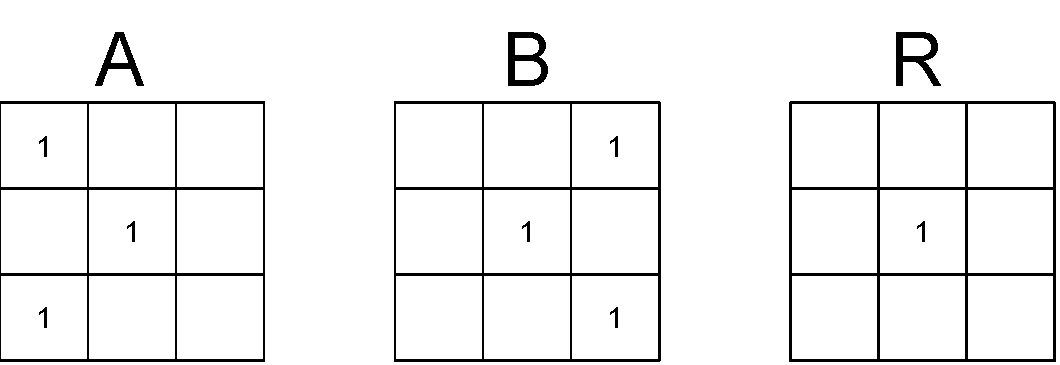
\includegraphics[width=0.7\textwidth]{images/routine-numbers-1.pdf}
    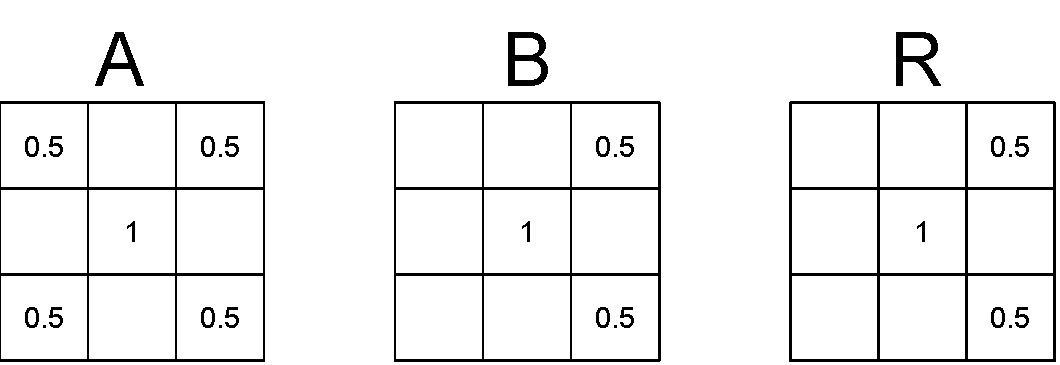
\includegraphics[width=0.7\textwidth]{images/routine-numbers-2.pdf}
    \caption{Two examples of the overlap function}
    \label{fig:routine-matrix-example}
\end{figure}

For the first matrix, using Equation \eqref{eq:feature-routine-index}, the Routine Index becomes:

\begin{equation}
RI = \frac{1}{1 + 1 + 1} = \frac{1}{3}
\end{equation}

For the second matrix, using Equation \eqref{eq:feature-routine-index}, the Routine Index becomes:

\begin{equation}
RI = \frac{1 + 2\cdot 0.5}{2} = 1
\end{equation}

